%%%%%%%%%%%%%%%%%%%%%%%%%%%%%%%%%%%%%%%%%%%%%%%%%%%%%%%%
\documentclass[12pt,a4paper]{article}% 文档格式
\usepackage{ctex,hyperref}% 输出汉字
\usepackage{times}% 英文使用Times New Roman
%%%%%%%%%%%%%%%%%%%%%%%%%%%%%%%%%%%%%%%%%%%%%%%%%%%%%%%%
\title{\fontsize{18pt}{27pt}\selectfont% 小四字号,1.5倍行距
    {\heiti% 黑体
        计算物理——Homework Week 14}}% 题目
%%%%%%%%%%%%%%%%%%%%%%%%%%%%%%%%%%%%%%%%%%%%%%%%%%%%%%%%
\author{\fontsize{12pt}{18pt}\selectfont% 小四字号,1.5倍行距
    {\fangsong% 仿宋
        白博臣、何骐多、夏营}\\% 标题栏脚注
    \fontsize{10.5pt}{15.75pt}\selectfont% 五号字号,1.5倍行距
    {\fangsong% 仿宋
        (四川大学~~~物理学拔尖计划)}}% 作者单位,“~”表示空格
%%%%%%%%%%%%%%%%%%%%%%%%%%%%%%%%%%%%%%%%%%%%%%%%%%%%%%%%
\date{}% 日期(这里避免生成日期)
%%%%%%%%%%%%%%%%%%%%%%%%%%%%%%%%%%%%%%%%%%%%%%%%%%%%%%%%
\usepackage{amsmath,amsfonts,amssymb}% 为公式输入创造条件的宏包
%%%%%%%%%%%%%%%%%%%%%%%%%%%%%%%%%%%%%%%%%%%%%%%%%%%%%%%%
\usepackage{graphicx}% 图片插入宏包
\usepackage{subfigure}% 并排子图
\usepackage{float}% 浮动环境,用于调整图片位置
\usepackage[export]{adjustbox}% 防止过宽的图片
%%%%%%%%%%%%%%%%%%%%%%%%%%%%%%%%%%%%%%%%%%%%%%%%%%%%%%%%
\usepackage{bibentry}
\usepackage{natbib}% 以上2个为参考文献宏包
%%%%%%%%%%%%%%%%%%%%%%%%%%%%%%%%%%%%%%%%%%%%%%%%%%%%%%%%
\usepackage{abstract}% 两栏文档,一栏摘要及关键字宏包
\renewcommand{\abstracttextfont}{\fangsong}% 摘要内容字体为仿宋
\renewcommand{\abstractname}{\textbf{摘\quad 要}}% 更改摘要二字的样式
%%%%%%%%%%%%%%%%%%%%%%%%%%%%%%%%%%%%%%%%%%%%%%%%%%%%%%%%
\usepackage{xcolor}% 字体颜色宏包
\newcommand{\red}[1]{\textcolor[rgb]{1.00,0.00,0.00}{#1}}
\newcommand{\blue}[1]{\textcolor[rgb]{0.00,0.00,1.00}{#1}}
\newcommand{\green}[1]{\textcolor[rgb]{0.00,1.00,0.00}{#1}}
\newcommand{\darkblue}[1]
{\textcolor[rgb]{0.00,0.00,0.50}{#1}}
\newcommand{\darkgreen}[1]
{\textcolor[rgb]{0.00,0.37,0.00}{#1}}
\newcommand{\darkred}[1]{\textcolor[rgb]{0.60,0.00,0.00}{#1}}
\newcommand{\brown}[1]{\textcolor[rgb]{0.50,0.30,0.00}{#1}}
\newcommand{\purple}[1]{\textcolor[rgb]{0.50,0.00,0.50}{#1}}% 为使用方便而编辑的新指令
%%%%%%%%%%%%%%%%%%%%%%%%%%%%%%%%%%%%%%%%%%%%%%%%%%%%%%%%
\usepackage{url}% 超链接
\usepackage{bm}% 加粗部分公式
\usepackage{multirow}
\usepackage{booktabs}
\usepackage{svg}
\usepackage{epstopdf}
\usepackage{epsfig}
\usepackage{longtable}% 长表格
\usepackage{supertabular}% 跨页表格
\usepackage{algorithm}
\usepackage{algorithmic}
\usepackage{changepage}% 换页
%%%%%%%%%%%%%%%%%%%%%%%%%%%%%%%%%%%%%%%%%%%%%%%%%%%%%%%%
\usepackage{enumerate}% 短编号
\usepackage{caption}% 设置标题
\captionsetup[figure]{name=\fontsize{10pt}{15pt}\selectfont Figure}% 设置图片编号头
\captionsetup[table]{name=\fontsize{10pt}{15pt}\selectfont Table}% 设置表格编号头
%%%%%%%%%%%%%%%%%%%%%%%%%%%%%%%%%%%%%%%%%%%%%%%%%%%%%%%%
\usepackage{indentfirst}% 中文首行缩进
\usepackage[left=2.50cm,right=2.50cm,top=2.80cm,bottom=2.50cm]{geometry}% 页边距设置
\renewcommand{\baselinestretch}{1.5}% 定义行间距(1.5)
%%%%%%%%%%%%%%%%%%%%%%%%%%%%%%%%%%%%%%%%%%%%%%%%%%%%%%%%
\usepackage{fancyhdr} %设置全文页眉、页脚的格式
\pagestyle{fancy}
\hypersetup{colorlinks=true,linkcolor=black}% 去除引用红框,改变颜色

%%%%%%%%%%%%%%%%%%%%%%%%%%%%%%%%%%%%%%%%%%%%%%%%%%%%%%%%
\newtheorem{theorem}{\indent 定理}[section]
\newtheorem{lemma}[theorem]{\indent 引理}
\newtheorem{proposition}[theorem]{\indent 命题}
\newtheorem{corollary}[theorem]{\indent 推论}
\newtheorem{definition}{\indent 定义}[section]
\newtheorem{example}{\indent 例}[section]
\newtheorem{remark}{\indent 注}[section]
\newenvironment{solution}{\begin{proof}[\indent\bf 解]}{\end{proof}}
\renewcommand{\proofname}{\indent\bf 证明}

%%%%%%%%%%%%%%%%%%%%%%%%%%%%%%%%%%%%%%%%%%%%%%%%%%%%%%%%

\begin{document}% 以下为正文内容
\maketitle% 产生标题,没有它无法显示标题
%%%%%%%%%%%%%%%%%%%%%%%%%%%%%%%%%%%%%%%%%%%%%%%%%%%%%%%%
\lhead{}% 页眉左边设为空
\chead{}% 页眉中间设为空
\rhead{}% 页眉右边设为空
\lfoot{}% 页脚左边设为空
\cfoot{\thepage}% 页脚中间显示页码
\rfoot{}% 页脚右边设为空
%%%%%%%%%%%%%%%%%%%%%%%%%%%%%%%%%%%%%%%%%%%%%%%%%%%%%%%%
\begin{figure}[h]
    \centering
    \begin{minipage}{0.32\textwidth}
        \centering
        \includegraphics[width=\linewidth]{bbc}
        \caption{白博臣}
        \label{白博臣照片}
    \end{minipage}\hfill
    \begin{minipage}{0.305\textwidth}
        \centering
        \includegraphics[width=\linewidth]{hqd}
        \caption{何骐多}
        \label{何骐多照片}
    \end{minipage}\hfill
    \begin{minipage}{0.32\textwidth}
        \centering
        \includegraphics[width=\linewidth]{xy}
        \caption{夏营}
        \label{夏营照片}
    \end{minipage}
\end{figure}

%    \begin{center}% 居中处理
%    {\textbf{Abstract}}% 英文摘要
%    \end{center}
%    \begin{adjustwidth}{1.06cm}{1.06cm}% 英文摘要内容
%        \hspace{1.5em}Attention!If you input "dif{}ferent", the computer will output "different", but if you input "dif\{\}ferent", the computer will output "dif{}ferent"
%    \end{adjustwidth}
\newpage% 从新的一页继续

\section{Problem 1}
\subsection{理论分析}
自由程满足一定范围内的均匀分布,$\lambda\in\left(\bar{\lambda}-\delta,\bar{\lambda}+\delta\right)$

以平均自由程为单位长度,取$\bar{lambda}=1$,则有:$\lambda \~ U(1-b,1+b)$,$\lambda$在区间(1-b,1+b)上服从均匀分布,其数字特征为:
\[E(\lambda)=1\]
\[D(\lambda)=\frac{b^2}{3}\]

由方差计算公式可得:
\[E(\lambda^2)=1+\frac{b^2}{3}\]
代入化简可得自由程服从一定范围的均匀分布时,方均根距离与平均自由程的比值满足:
\[\frac{d(n)_{rms}}{\bar{\lambda}}=\sqrt{n}\cdot \sqrt{1+\frac{b^2}{3}}\]

\begin{figure}[htbp]
    \centering
    \includegraphics[height=8cm]{P1_1.png}\label{fig:figure4}
    \caption{固定$\lambda$的3D random walk}
\end{figure}

代入不同的b值,有对应的理论曲线:
\begin{figure}[htbp]
    \centering
    \includegraphics[height=8cm]{理论曲线.jpg}\label{fig:figure4}
    \caption{理论曲线}
\end{figure}

\begin{figure}[htbp]
    \centering
    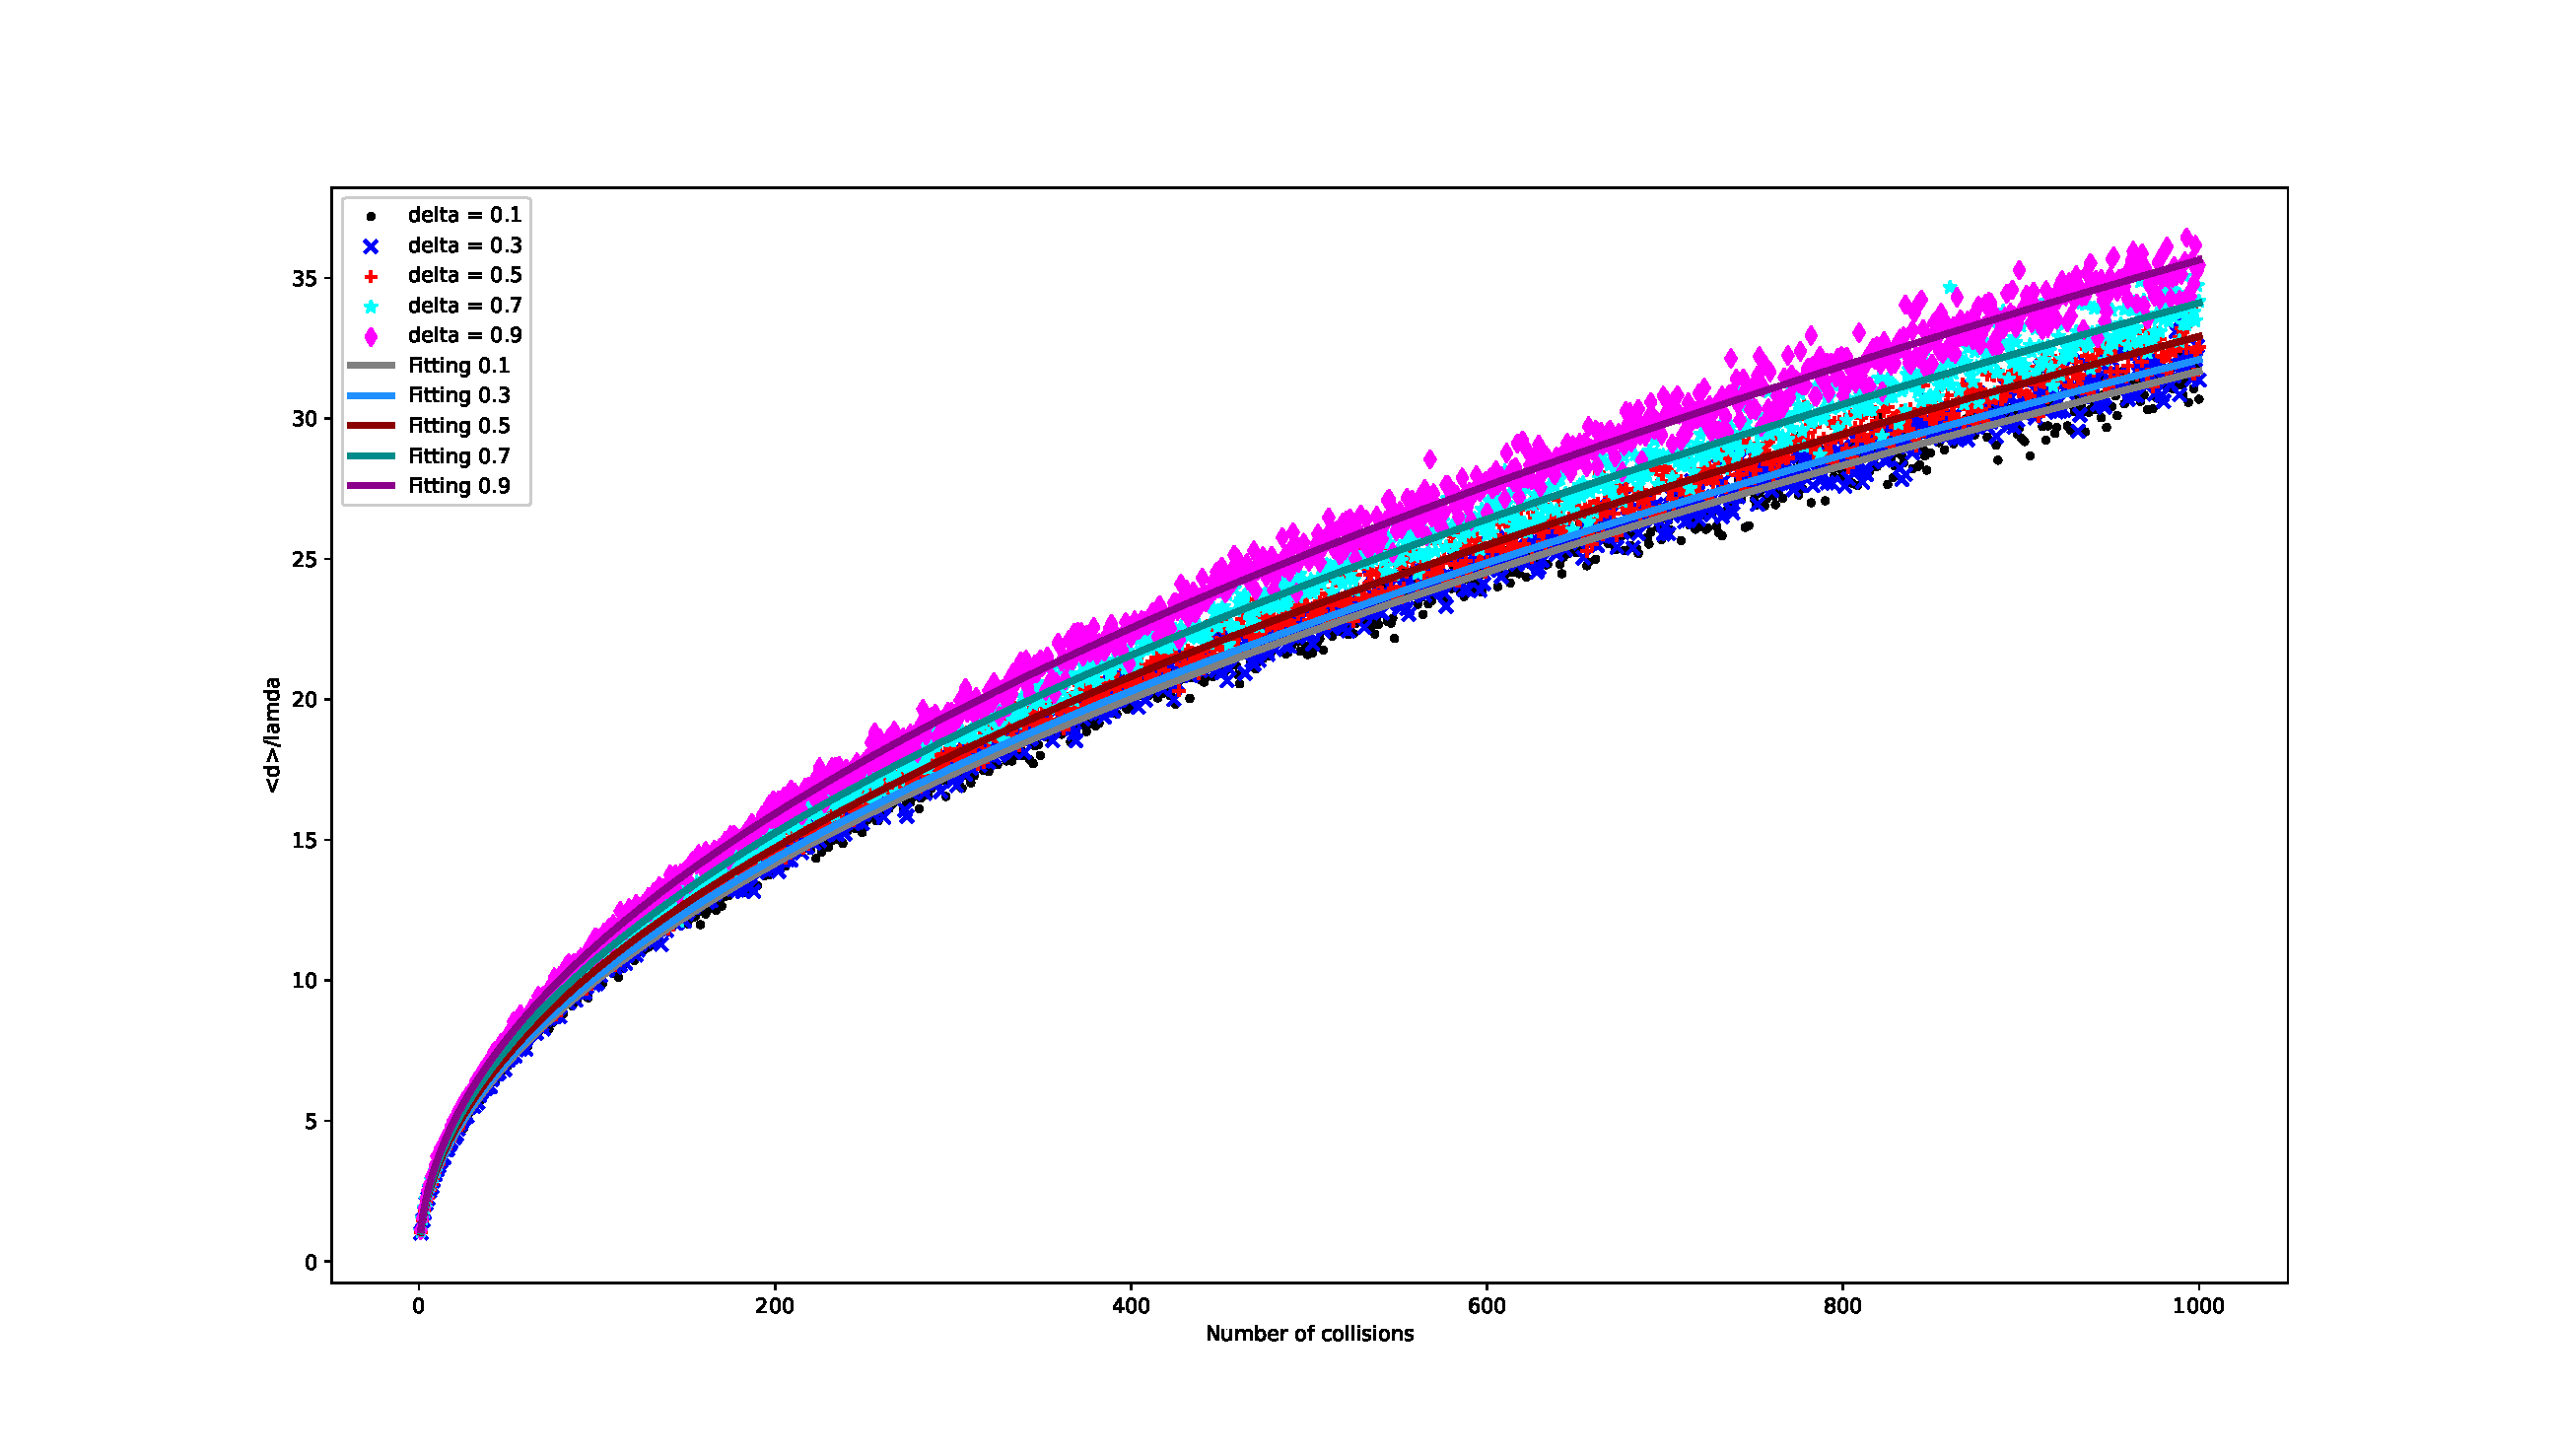
\includegraphics[height=8cm]{Figure_1.eps}\label{fig:figure4}
    \caption{不固定$\lambda$的3D random walk及其}
\end{figure}

我们可以发现点聚集整体可以有微小差异随着方差变大,整体有略微抬升,差异很明显,引入$\lambda$方差引起的预测偏差越大越明显将大部分点抬升至$\sqrt(N)$上面,原因就是方差引入一定程度的偏差。结果表明,拟合曲线和理论曲线几乎完全重合,进一步验证了理论推导的正确性!也可以观察到,参数𝑏的值越大,均方根距离的值相对会增大。

\section{Problem 2}
\subsection{题目回顾}
溶液中聚合物的一个简单模型将其视为一系列随机取向的片段:也就是说,一个片段的取向与任何其他片段的取向之间没有相关性。这就是所谓的随机飞行模型,或自由连接随机行走链模型。
\subsection{问题解答}
首先我们定义了一个名为Polymer的类,表示在溶液中的随机飞行聚合物。在类的初始化方法init中,传入N和a两个参数,分别表示聚合物的段数和每段的长度。之后,将N和a保存在self.N和self.a中,并创建一个长度为N的空列表self.xyz来保存聚合物的段位置向量。还定义了一个变量self.R来保存聚合物的端到端向量。make\_polymer方法用来计算随机飞行聚合物的段位置、质心和端到端距离。首先,将第一个段的位置设为原点(0,0,0)。然后,使用循环从第二个段开始逐个计算段的位置。每个段的位置由随机选择的角度theta和phi决定,通过计算对应的位移向量来更新当前位置。每次计算得到一个段的位置后,将其存储在self.xyz中,并更新质心的坐标。最后,计算质心的位置,并将最后一个段的位置作为端到端向量self.R。最后,calc\_Rg方法用来计算并返回聚合物的旋转半径Rg。该方法首先初始化self.Rg为0,然后遍历所有段的位置,计算每个段的坐标的平方和,并累加到self.Rg中。最后,将self.Rg除以N并取平方根,得到Rg的值,并返回它。

接着导入了一个名为Polymer的模块,并从该模块中导入了Polymer类。接下来,创建了一个名为polymer1的Polymer对象,传入了参数1000和0.5,表示创建一个由1000个长度为0.5的段组成的聚合物。然后,通过polymer1.R可以获取聚合物的端到端向量。最后,通过polymer1.calc\_Rg()可以计算聚合物的旋转半径Rg,并返回它的值:
\[R_g=6.276669088499813\]

定义了一个变量Np,表示要计算的聚合物数量,为3000。然后,通过循环计算了Np个聚合物的端到端距离R。每个聚合物由N个长度为a的段组成,并使用Polymer类创建了一个polymer对象。接着,计算并保存聚合物的端到端距离Rx、Ry、Rz,并将其存储在R列表中。使用plt.hist函数绘制了R的分布情况,使用50个bin来绘制,density=True来进行归一化。绘制了r和Pr的曲线见下图:
\begin{figure}[htbp]
    \centering
    \includegraphics[height=8cm]{p2_1.png}\label{fig:figure4}
    \caption{P(R)与R关系图}
\end{figure}

\section{Problem 3}
\subsection{问题解答}
\subsubsection{问题a解答}
模拟一维轴上行走,每步决定一次向左/向右,各有一次0.5概率选择-1,+1。
\begin{figure}[htbp]
    \centering
    \includegraphics[height=8cm]{P3_1.png}\label{fig:figure4}
    \caption{P(R)与R关系图}
\end{figure}

通过改变N值,得到不同N值下的随机行走:

\begin{figure}[H]% 插入两张图片并且并排
    \centering
    \begin{minipage}{0.48\textwidth}
        \centering
        \includegraphics[width=1.1\textwidth]{128.1.png}
        \caption{\fontsize{10pt}{15pt}\selectfont N=128}
    \end{minipage}
    \hspace{0cm}% 图片间距
    \hfill% 撑满整行
    \begin{minipage}{0.48\textwidth}
        \centering
        \includegraphics[width=1.1\textwidth]{128.png}
        \caption{\fontsize{10pt}{15pt}\selectfont N=128}
    \end{minipage}\label{fig:figure3}
\end{figure}

\begin{figure}[H]% 插入两张图片并且并排
    \centering
    \begin{minipage}{0.48\textwidth}
        \centering
        \includegraphics[width=1.1\textwidth]{256.2.png}
        \caption{\fontsize{10pt}{15pt}\selectfont N=256}
    \end{minipage}
    \hspace{0cm}% 图片间距
    \hfill% 撑满整行
    \begin{minipage}{0.48\textwidth}
        \centering
        \includegraphics[width=1.1\textwidth]{256.png}
        \caption{\fontsize{10pt}{15pt}\selectfont N=256}
    \end{minipage}\label{fig:figure3}
\end{figure}

\begin{figure}[H]% 插入两张图片并且并排
    \centering
    \begin{minipage}{0.48\textwidth}
        \centering
        \includegraphics[width=1.1\textwidth]{512.2.png}
        \caption{\fontsize{10pt}{15pt}\selectfont N=512}
    \end{minipage}
    \hspace{0cm}% 图片间距
    \hfill% 撑满整行
    \begin{minipage}{0.48\textwidth}
        \centering
        \includegraphics[width=1.1\textwidth]{512.png}
        \caption{\fontsize{10pt}{15pt}\selectfont N=512}
    \end{minipage}\label{fig:figure3}
\end{figure}

\begin{figure}[H]% 插入两张图片并且并排
    \centering
    \begin{minipage}{0.48\textwidth}
        \centering
        \includegraphics[width=1.1\textwidth]{1024.1.png}
        \caption{\fontsize{10pt}{15pt}\selectfont N=1024}
    \end{minipage}
    \hspace{0cm}% 图片间距
    \hfill% 撑满整行
    \begin{minipage}{0.48\textwidth}
        \centering
        \includegraphics[width=1.1\textwidth]{1024.png}
        \caption{\fontsize{10pt}{15pt}\selectfont N=1024}
    \end{minipage}\label{fig:figure3}
\end{figure}

能够观察到拟合效果较好,可以近似认为符合正太分布。

我们发现,在N值改变的过程中,P的最大值式中在$X=0$处取得,在$X=25 and X=-25$附近P值会逐渐趋向于0.

当改为向左频率为0.7的时候,我们可以得到如下分布:
\begin{figure}[htbp]
    \centering
    \includegraphics[height=2cm]{P3_2.jpg}\label{fig:figure4}
    \caption{向左频率为0.7时的分布}
\end{figure}

观察以向左的概率为0.7得到的分布,可以看出平均位置是在-40左右,均方差是在40左右。

\section{Problem 4}
\subsection{问题回顾}
\textbf{二维随机行走}:聚合物是由几个重复亚基(单体)组成的大分子。它们在我们的日常生活中发挥着重要作用,从生物过程到合成材料。在这里,我们模拟了线性和无支链的聚合物,它们浸泡在良好的溶剂中。
\subsection{问题解答}
分别采用2D Sample Random Walk , 2D Traditional Random Walk , 2D Self-Avoiding Random Walk来计算双端距离$<R_e^2>$和回旋半径$<R_g^2$,并且绘制其对数值与步数的值的关系图,并对其进行线性拟合。

对于\textbf{2D Sample Random Walk}:

\begin{figure}[htbp]
    \centering
    \includegraphics[height=7cm]{P4_1.1.png}\label{fig:figure4}
    \caption{$<R_e^2>$对数关系图}
\end{figure}

\begin{figure}[htbp]
    \centering
    \includegraphics[height=7cm]{p4_1.2.png}\label{fig:figure4}
    \caption{$<R_g^2>$对数关系图}
\end{figure}

\newpage

\textbf{2D Traditional Random Walk}:

\begin{figure}[htbp]
    \centering
    \includegraphics[height=7cm]{P4_2.1.png}\label{fig:figure4}
    \caption{$<R_e^2>$对数关系图}
\end{figure}

\begin{figure}[htbp]
    \centering
    \includegraphics[height=7cm]{p4_2.2.png}\label{fig:figure4}
    \caption{$<R_g^2>$对数关系图}
\end{figure}

\newpage

\textbf{2D Self-Avoiding Random Walk}:

\begin{figure}[htbp]
    \centering
    \includegraphics[height=7cm]{P4_4.1.png}\label{fig:figure4}
    \caption{$<R_e^2>$对数关系图}
\end{figure}

\begin{figure}[htbp]
    \centering
    \includegraphics[height=7cm]{p4_4.2.png}\label{fig:figure4}
    \caption{$<R_g^2>$对数关系图}
\end{figure}

通过绘图与拟合我们发现自回避随机行走的线性拟合为:$y=1.32x+0.05$,对应得到$\nu=0.66$,与理论值3/4较为接近。
\newpage

\section{Problem 5}
3D Random Walk 中的Traditional方法与Problem 1过程思路一致,此处不再冗余阐述。

对于3D Self-Avoiding Random Walk ,同Problem 4 处理,得到以下图像:

\begin{figure}[htbp]
    \centering
    \includegraphics[height=8cm]{P5_1.png}\label{fig:figure4}
    \caption{$<R_g^2>$对数关系图}
\end{figure}

得到的斜率为$\nu=0.52$与理论值0.6较为接近!

\end{document}